%\documentclass[fontsize=12pt, paper=a4]{report}
\documentclass[fontsize=12pt, paper=a4]{scrreprt}
%\documentclass[fontsize=12pt, paper=a4, headinclude, twoside=false, parskip=half+, pagesize=auto, numbers=noenddot, plainheadsepline, open=right]{scrreprt}
%\documentclass[11pt,a4paper]{article}
%\usepackage[latin1]{inputenc}
\usepackage[utf8]{inputenc}
\usepackage[T1]{fontenc}
%\usepackage[ngerman]{babel}
\usepackage[ngerman,english]{babel}
\usepackage[square,numbers]{natbib}
\usepackage{textcomp}
\usepackage{lmodern}

\usepackage[intlimits]{amsmath}
\usepackage{amssymb}
\usepackage{moreverb}

% PDF-Kompression
\pdfminorversion=5
\pdfobjcompresslevel=1

%\usepackage[automark]{scrpage2} % Kopf- und Fu�zeilen
%\usepackage{amsmath,marvosym} % Mathesachen
%\usepackage{mathpazo} % Palatino f�r Mathemodus
%\usepackage{mathpazo,tgpagella} % auch sehr sch�ne Schriften

\usepackage{setspace} % Zeilenabstand
\onehalfspacing % 1,5 Zeilen

% Schriften-Gr��en
\setkomafont{chapter}{\Large\rmfamily}
\setkomafont{section}{\large\rmfamily}
\setkomafont{subsection}{\normalsize\rmfamily}
\setkomafont{subsubsection}{\normalsize\rmfamily}
\setkomafont{paragraph}{\rmfamily}
\setkomafont{subparagraph}{\rmfamily}
%\setkomafont{chapterentry}{\large\rmfamily}
%\setkomafont{descriptionlabel}{\bfseries\rmfamily}
\setkomafont{captionlabel}{\upshape\bfseries}
\setkomafont{caption}{\itshape}

\usepackage[ngerman,english,pdfauthor={Andreas Mantler}, pdftitle={Design of a Semi-Actuated Tangible Device for Tabletop Interface Interactions}, breaklinks=true]{hyperref}
\usepackage[final]{microtype}
\usepackage{url}
\usepackage{multirow}
\usepackage{multicol}
\usepackage{tabularx}
\usepackage{longtable}
\usepackage{array}
\usepackage{float}
\usepackage{graphicx}
\usepackage{color}

\graphicspath{{images/}}
\DeclareGraphicsExtensions{.pdf,.png,.jpg}
\renewcommand{\thefigure}{\arabic{figure}}
\renewcommand{\thetable}{\arabic{table}}
\usepackage{subcaption}
\usepackage{rotating}
%\newcommand{\subfigureautorefname}{\figurename}
\usepackage[all]{hypcap}
%\setcapindent{0em}
%\setcapwidth[c]{0.9\textwidth}
%\setlength{\abovecaptionskip}{0.2cm}
\usepackage{chngcntr}
\counterwithout{figure}{chapter}

\usepackage{listings}
\usepackage{color}

\definecolor{mycomment}{rgb}{0,0.6,0}
\definecolor{mygray}{rgb}{0.5,0.5,0.5}
\definecolor{mymauve}{rgb}{0.58,0,0.22}

\lstset{ %
  backgroundcolor=\color{white},   % choose the background color; you must add \usepackage{color} or \usepackage{xcolor}
  basicstyle=\footnotesize,        % the size of the fonts that are used for the code
  breakatwhitespace=false,         % sets if automatic breaks should only happen at whitespace
  breaklines=true,                 % sets automatic line breaking
  commentstyle=\color{mycomment},  % comment style
  deletekeywords={...},            % if you want to delete keywords from the given language
  escapeinside={\%*}{*)},          % if you want to add LaTeX within your code
  extendedchars=true,              % lets you use non-ASCII characters; for 8-bits encodings only, does not work with UTF-8
  frame=single,                    % adds a frame around the code
  keepspaces=true,                 % keeps spaces in text, useful for keeping indentation of code (possibly needs columns=flexible)
  keywordstyle=\color{blue},       % keyword style
  language=C++,                    % the language of the code
%  otherkeywords={*,...},           % if you want to add more keywords to the set
  numbers=left,                    % where to put the line-numbers; possible values are (none, left, right)
  numbersep=5pt,                   % how far the line-numbers are from the code
  numberstyle=\tiny\color{mygray}, % the style that is used for the line-numbers
  rulecolor=\color{black},         % if not set, the frame-color may be changed on line-breaks within not-black text (e.g. comments (green here))
  showspaces=false,                % show spaces everywhere adding particular underscores; it overrides 'showstringspaces'
  showstringspaces=false,          % underline spaces within strings only
  showtabs=false,                  % show tabs within strings adding particular underscores
  stepnumber=1,                    % the step between two line-numbers. If it's 1, each line will be numbered
  stringstyle=\color{mymauve},     % string literal style
  tabsize=2,                       % sets default tabsize to 2 spaces
  title=\lstname                   % show the filename of files included with \lstinputlisting; also try caption instead of title
}
%\lstset{
%	extendedchars=true,
%	basicstyle=\tiny\ttfamily,
%	tabsize=2,
%	keywordstyle=\textbf,
%	commentstyle=\color{gray},
%	stringstyle=\textit,
%	numbers=left,
%	numberstyle=\tiny,
%	breakautoindent  = true,
%	breakindent      = 2em,
%	breaklines       = true,
%	postbreak        = ,
%	prebreak         = \raisebox{-.8ex}[0ex][0ex]{\Righttorque},
%}

% linksb�ndige Fu�boten
\deffootnote{1.5em}{1em}{\makebox[1.5em][l]{\thefootnotemark}}

\typearea{14}

\makeatletter
\newcommand{\saved@equation}{}
\let\saved@equation\equation
\def\equation{\@hyper@itemfalse\saved@equation}
\makeatother

% einr�cken nach �berschriften
\makeatletter
\let\@afterindentfalse\@afterindenttrue % Absatzeinzug auch nach �berschriften
\@afterindenttrue
\makeatother

\newcommand*\justify{%
  \fontdimen2\font=0.4em% interword space
  \fontdimen3\font=0.2em% interword stretch
  \fontdimen4\font=0.1em% interword shrink
  \fontdimen7\font=0.1em% extra space
  \hyphenchar\font=`\-% allowing hyphenation
}

% bild mit defnierter Breite einf�gen
\newcommand{\bild}[4]{
  \begin{figure}[!hbt]
    \centering
      \vspace{1ex}
      \includegraphics[width=#2]{images/#1}
      \caption[#4]{\label{img.#1} #3}
    \vspace{1ex}
  \end{figure}
}
% bild mit eigener Breite
\newcommand{\bilda}[3]{
  \begin{figure}[!hbt]
    \centering
      \vspace{1ex}
      \includegraphics{images/#1}
      \caption[#3]{\label{img.#1} #2}
      \vspace{1ex}
  \end{figure}
}

\font\texttrm = cmr17
\font\textttrm = cmr17 at 13pt

\addtolength{\textwidth}{-15mm}
\addtolength{\oddsidemargin}{13mm}

\addtolength{\headheight}{6.5mm}
\addtolength{\headsep}{0mm}%-24.5mm}
\addtolength{\textheight}{5mm}%28.5mm}
\addtolength{\footskip}{-7.5mm}

\usepackage[headsepline, footsepline, plainheadsepline]{scrpage2}
\pagestyle{scrheadings}
\clearscrheadfoot
\renewcommand*{\chaptermarkformat}{}
%\renewcommand*{\sectionmarkformat}{}
\automark[section]{chapter}
\renewcommand*{\chapterheadstartvskip}{\vspace{-11mm}}
\renewcommand*{\chapterheadendvskip}{\vspace{4mm}}

\setlength{\parindent}{0mm}

% punkte im Inhaltsverzeichnis
\makeatletter
\renewcommand*\l@chapter[2]{
  \ifnum \c@tocdepth >\m@ne
    \addpenalty{-\@highpenalty}
    \vskip 1.0em \@plus\p@
    \setlength\@tempdima{1.5em}
    \begingroup
      \parindent \z@ \rightskip \@pnumwidth
      \parfillskip -\@pnumwidth
      \leavevmode \bfseries
      \advance\leftskip\@tempdima
      \hskip -\leftskip
      #1\nobreak\normalfont\leaders\hbox{$\m@th
        \mkern \@dotsep mu\hbox{.}\mkern \@dotsep
        mu$}\hfill\nobreak\hb@xt@\@pnumwidth{\hss\bf #2}\par
      \penalty\@highpenalty
    \endgroup
  \fi}

%\renewcommand\l@section[2]{
%  \ifnum \c@tocdepth >\z@
%    \addpenalty\@secpenalty
%    \addvspace{1.0em \@plus\p@}
%    \setlength\@tempdima{1.5em}
%    \begingroup
%      \parindent \z@ \rightskip \@pnumwidth
%      \parfillskip -\@pnumwidth
%      \leavevmode \bfseries
%      \advance\leftskip\@tempdima
%      \hskip -\leftskip
%      #1\nobreak\ 
%      \leaders\hbox{$\m@th\mkern \@dotsep mu\hbox{.}\mkern \@dotsep mu$}
%     \hfil \nobreak\hb@xt@\@pnumwidth{\hss #2}\par
%    \endgroup
%  \fi}
%\makeatother

% newline after \paragraph
\makeatletter
\renewcommand\paragraph{%
   \@startsection{paragraph}{4}{0mm}%
      {-\baselineskip}%
      {.01\baselineskip}%
      {\normalfont\normalsize\bfseries}}
\makeatother

\AtBeginDocument{\addtocontents{toc}{\protect\thispagestyle{empty}}}



\begin{document}

	% Titelseite
	\begin{center}
		\vspace*{54mm}
		{
			\renewcommand{\baselinestretch}{0.9}\normalsize
			\Large
			\textbf{Oculus Meets AR - Documentation}\\
		}
		\vspace*{15.5mm}
		{
			\large
			\textbf{Project Seminar}\\
		}
		\vspace*{10mm}
		{
			at\\
			\textbf{Westfälischen Wilhelms-Universität Münster}\\
		}
		\vspace*{100mm}
		\begin{tabular*}{137mm}{ll}
			Authors: 		& \textbf{Tim Michels }, Matr.Nr. \\
						& \textbf{Florian Kleene}, Matr.Nr. 374601\\
						& \textbf{Christian Thiele}, Matr.Nr. \\
						& \textbf{Andreas Mantler}, Matr.Nr. 363220\\
			Submission date: 	& April 20th 2015
		\end{tabular*}
	\end{center}
	\newpage
	
	% Leere Seite
	\thispagestyle{empty}\quad\newpage
	
	% Inhaltsverzeichnis
	\thispagestyle{empty}
	\tableofcontents
	\addtocontents{toc}{\vspace{-5mm}}
	\vfill
	\newpage

	% Leere Seite
	\thispagestyle{empty}\quad\newpage
	
	% Inhalt
	\setcounter{page}{1}
	\pagestyle{scrheadings}
	\setfootsepline{0pt} 
	\ihead[\chaptername\ \thechapter: \leftmark]{\chaptername\ \thechapter: \leftmark}
	\cfoot[\vspace*{9mm}\pagemark]{\vspace*{9mm}\pagemark}
	\renewcommand{\baselinestretch}{1.3}\normalsize

	\chapter{Introduction}
	\label{sec:introduction}
	The aim of this project is to equip the Oculus Rift DK2 with a stereo camera system and build a framework in order to extend its functionality regarding AR (augmented reality). While AR applications using smartphones or wearables like Google Glass are only able to augment a small part of our FOV (field of view), head mounted displays (HMD) like Oculus Rift are not limited in this regard and are therefore creating a more immersive experience. Furthermore the use of a HMD enables the user to switch between VR (virtual reality) and AR.\\
In addition we integrate a tracking system, which enables us to get the exact position of the HMD as well as the position of any other object equipped with so-called rigid bodies. This allows interactions with the virtual objects supplemented to the real-world environment without using further input devices.

\section*{Previous Work}
There are mainly two similar (published) projects to ours. The first one is the commercial \href{http://ovrvision.com/}{OVRVision} by Shinobiya.com Co.Ltd., which is available for Oculus Rift DK2. The OVRVision has two fixed, parallel mounted cameras and therefore lacks the option to adjust the position of these cameras to match the user's IPD (interpupillary distance). Secondly there is William Steptoe's well documented project \href{http://willsteptoe.com/post/66968953089/ar-rift-part-1}{AR-Rift}, which is more flexible regarding the cameras' positions, but is based on the Oculus Rift DK1, which has a much lower resolution than the DK2 used for our project. Nevertheless our project is built upon ideas of both these AR-extensions for Oculus Rift.	

	\chapter{Hardware Requirements}
	\label{sec:hardware_requirements}
	Please note that every single part of the following hardware
configuration is optional in the example applications. You do not need
any of the hardware present to develop with ARLib! This is the hardware we were
developing for:
\begin{itemize}
	\item{2x \href{http://www.logitech.com/de-de/product/hd-webcam-c310}{Logitech C310 Webcams}}
	\item{\href{https://github.com/ands/OculusMeetsAR/tree/master/Hardware/Printmodels}{3D-Printed camera mounts and lens mounts}}
	\item{2x \href{http://www.camera2000.com/en/cctv-board-security-video-camera-1-8mm-lens-f2-0.html}{Fisheye 1.8mm lens F2.0}}
	\item{\href{https://www.oculus.com/dk2/}{Oculus Rift DK2 Head-Mounted Display}}
	\item{\href{http://www.optitrack.com/products/flex-3/}{OptiTrack Flex 3 Tracking System}}
\end{itemize}

\begin{figure}[htb!]
	\centering
	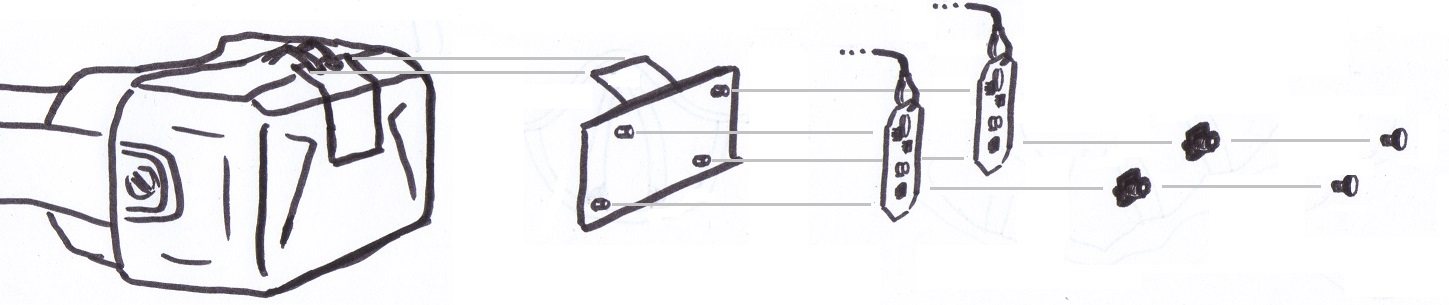
\includegraphics{explosion}
	\vspace{1mm}
	\caption{Exploded-view drawing of our modified HMD. The components from left to right: Oculus Rift DK2, 3D-printed camera mount, Logitech C310s, 3D-printed lens mounts, lenses.}
	\label{fig:explosion}
\end{figure}

\subsection{Lens selection and camera calibration}\label{lens-selection-and-camera-calibration}

Regarding our hardware choices we recommend William Steptoe's
\href{http://willsteptoe.com/post/67399683294/ar-rift-camera-selection-part-2}{documentation
on his project AR-Rift}. According to different user-reports, the actual
horizontal FOV of the DK2, which should be matched by the lenses, is
only about 80\textdegree-90\textdegree. With our lenses, we got a vertical* FOV of
approximately 75\textdegree, so for a more accurate matching one might want to buy
lenses with a smaller focal length. To prevent easy mistakes on your
search for other lenses, we recommend
\href{http://pomeroyprinting.blogspot.de/2014/04/modifying-logitech-c310-hd-webcam.html}{this
post by Brandon Pomeroy}.

For calibration we used Davide Scaramuzzas
\href{https://sites.google.com/site/scarabotix/ocamcalib-toolbox}{OCamCalib toolbox} along with a small
\href{https://github.com/ands/OculusMeetsAR/tree/master/Hardware}{stereo calibration tool}, we implemented using OpenCV. Click
\href{https://github.com/ands/OculusMeetsAR/wiki/Calibration}{here} for a step-by-step guide and technical details.
\\
\\
*Remark: This is the relevant FOV since the cameras are mounted with a 90\textdegree rotation!
	
	\chapter{Tracking Library}
	\label{sec:tracking_library}
	\begin{center}
\textbf{Developed by Florian Kleene \& Christian Thiele}
\end{center}
The Tracking Library supports several methods for real-time pose determination and estimation. Along with the tracking devices included in the Oculus Rift (both DK1 and DK2\cite{dk2}), any device using the NatNetSDK\cite{optitrack} is supported. The core of this Module is the \texttt{TrackingManager} class. It is practically the only necessary interface to fire-up an application with tracking support. The proper use of the tracking library will be discussed in the following sections.
\section{Initialization of the Tracking Manager}\label{tracking-manager-initialization}

Initialization of the tracking manager requires the user to hand over the necessary parameters to the TrackingManager beforehand. First of all we create an instance of the class while also defining its purpose.

\begin{lstlisting}
TrackingManager tManager = TrackingManager(ARLib::ARLIB_NATNET | ARLib::ARLIB_RIFT, frameBufferSize, debugOutput);
\end{lstlisting}
where frameBufferSize determines the buffer size for retroactive queries (more on that later) and debugOutput is a boolean value enabling debug console output. In this example the tracking manager is set up to connect to a NatNet Server (i.e Motive etc.) as well as reading tracking data from the rifts inertial sensors, providing more stability in the tracking data (there is also support for multiple rifts).
The \texttt{initialize} function returns the status of the tracking manager. This is very helpfull for debugging. Furthermore the tracking manager should not be used unless no error is returned by the \texttt{initialize} function.

\begin{lstlisting}
if(ARLib::ARLIB_TRACKING_OK != tManager->initialize()){
    printf("Failed to Initialize Tracking Manager.");
    return -1;
}
\end{lstlisting}
Depending on wether the tracking is critical for your application or not you should exit your program.

\section{Using the Tracking Manager}\label{using-the-tracking-manager}

The tracking manager needs to be updated on a regular basis (i.e. your event-loop), if your are using the Oculus Rift. For smooth transformations, this should happen at least 75 times per second, that is the frame rate supported by the Oculus DK2, or 60 times per second for the DK1.

To make objects behave according to the tracking data (i.e. ridig body transformations) they have to inherit from the abstract base class \texttt{RigidBodyEventListener}. On each event cycle the manager will notify its listeners of any change in their transformations. A \texttt{RigidBodyEventListener} has a, not necessarily unique, ID, which is used to create a correspondence between the rigid bodies on the server (Motive etc.) and the rigid bodies in your application.

For the Oculus there is a specialized \texttt{RigidBodyEventListener} the \texttt{\justify RiftRigidBodyEventListener}. The \texttt{RiftSceneNode} from the OgreModule is such a specialized listener. On Registration with the Tracking Manager, a handle to the rift is saved and queried for positional data each frame.


\section{Retroactive Queries}\label{retroactive-queries}

The camera images need to be placed in front of the virtual camera, which is of course a representative of the Oculus. But to reduce the effect of latency, which is naturally imposed by the webcams, the images need to be placed where they were at capture time. This solution works rather nicely in situations where the camera motion is not particularly fast. When the camera is moving faster the user will experience black borders at the edge of the screen, because the images could not cover the whole rendering area. To query the position of the RiftRigidBodyEventListener one must call the function.

\begin{lstlisting}
RigidBody* TrackingManager::evaluateRigidBody(unsigned int ID, const long long& retroActiveQuery);
\end{lstlisting}

ID is of course the RigidBody identifier, and retroActiveQuery is the desired Timestamp formated equavalently to the QueryPerformanceCounter function.

\section{Cleaning Up}\label{cleaning-up}

If the Tracking Manager is no longer used simply delete the handle to it. The cleanup will be taken care of by the destructor.	
	
	% other content
	
%	\newpage

	% Quellenverzeichnis
%	\nocite{*}
%	\addcontentsline{toc}{chapter}{Bibliography}
%	\ihead[\leftmark]{\leftmark}
%	\begin{thebibliography}{99}

%	\end{thebibliography}
	
%	\newpage

\end{document}
